\documentclass{article}
\usepackage[a4paper, total={6.5in, 10.5in}]{geometry}
\usepackage{graphicx}

\author{Katarzyna Macioszek, Ada Majchrzak}
\title{Data Mining project - part II}

\begin{document}
	\maketitle
	
	\section{Introduction}
	In the second part of the project we will use clustering analysis in connection with dimension reduction methods on \textit{Spambase} dataset. Our goal is to asses clustering algorithms performance in differentiation between \textit{spam} and \textit{nonspam} types. For that we shall use \textit{k-means}, PAM and AGNES clustering algorithms. We will also check separation measures of clusters built using original data and data after dimension reduction done with PCA algorithm. Additionally we will also compare clustering results with classification methods performed on the former part of the project.
	
	\section{Data preparation}
	To be consistent with analysis done in previous part of the project we again exclude columns that exhibit high correlation with each other. In this eliminated features are \textit{num415} and \textit{num857}. Furthermore we also use the same data transformations: z-score standardization and $\log(x+0.1)$ transformation to make the explanatory variables have comparable values, as it is crucial for clustering and dimension reduction algorithms.
	
	\section{PCA}
	To be able to visualize the multidimensional data easily, we start with performing the principal component analysis (PCA). As mentioned before we use two data transformations, however to display an interesting behavior of the method let  us first present the outputs for non-transformed data. To visualize PCA results we will use scree plot and contributions of variables in first two principal components.
	
	\begin{figure}[h]
		\caption{PCA results for original data}
		\centering
		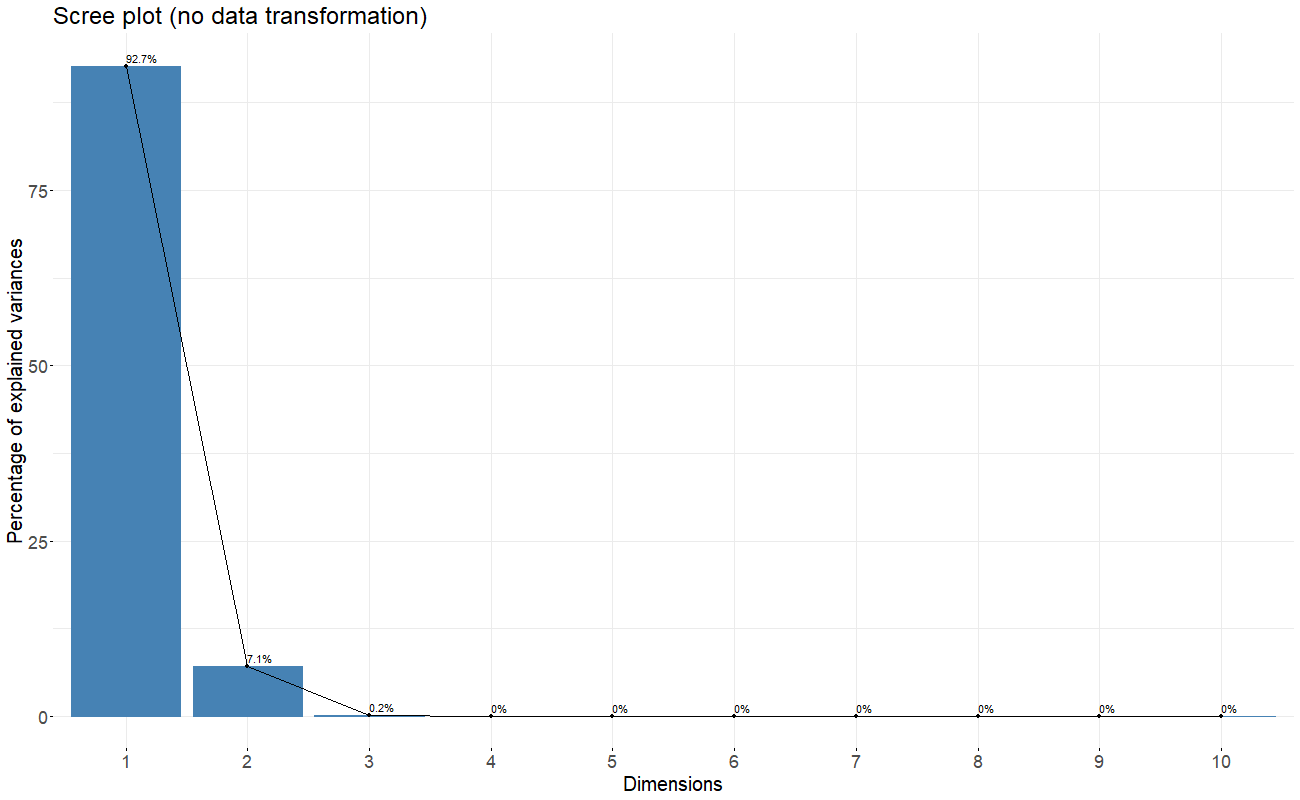
\includegraphics[width=0.7\textwidth]{"proj2_plots/screeplot1.png"}
		\label{fig::screeplot}
	\end{figure}
	
	\begin{figure}[h]
		\caption{PCA results for original data}
		\centering
		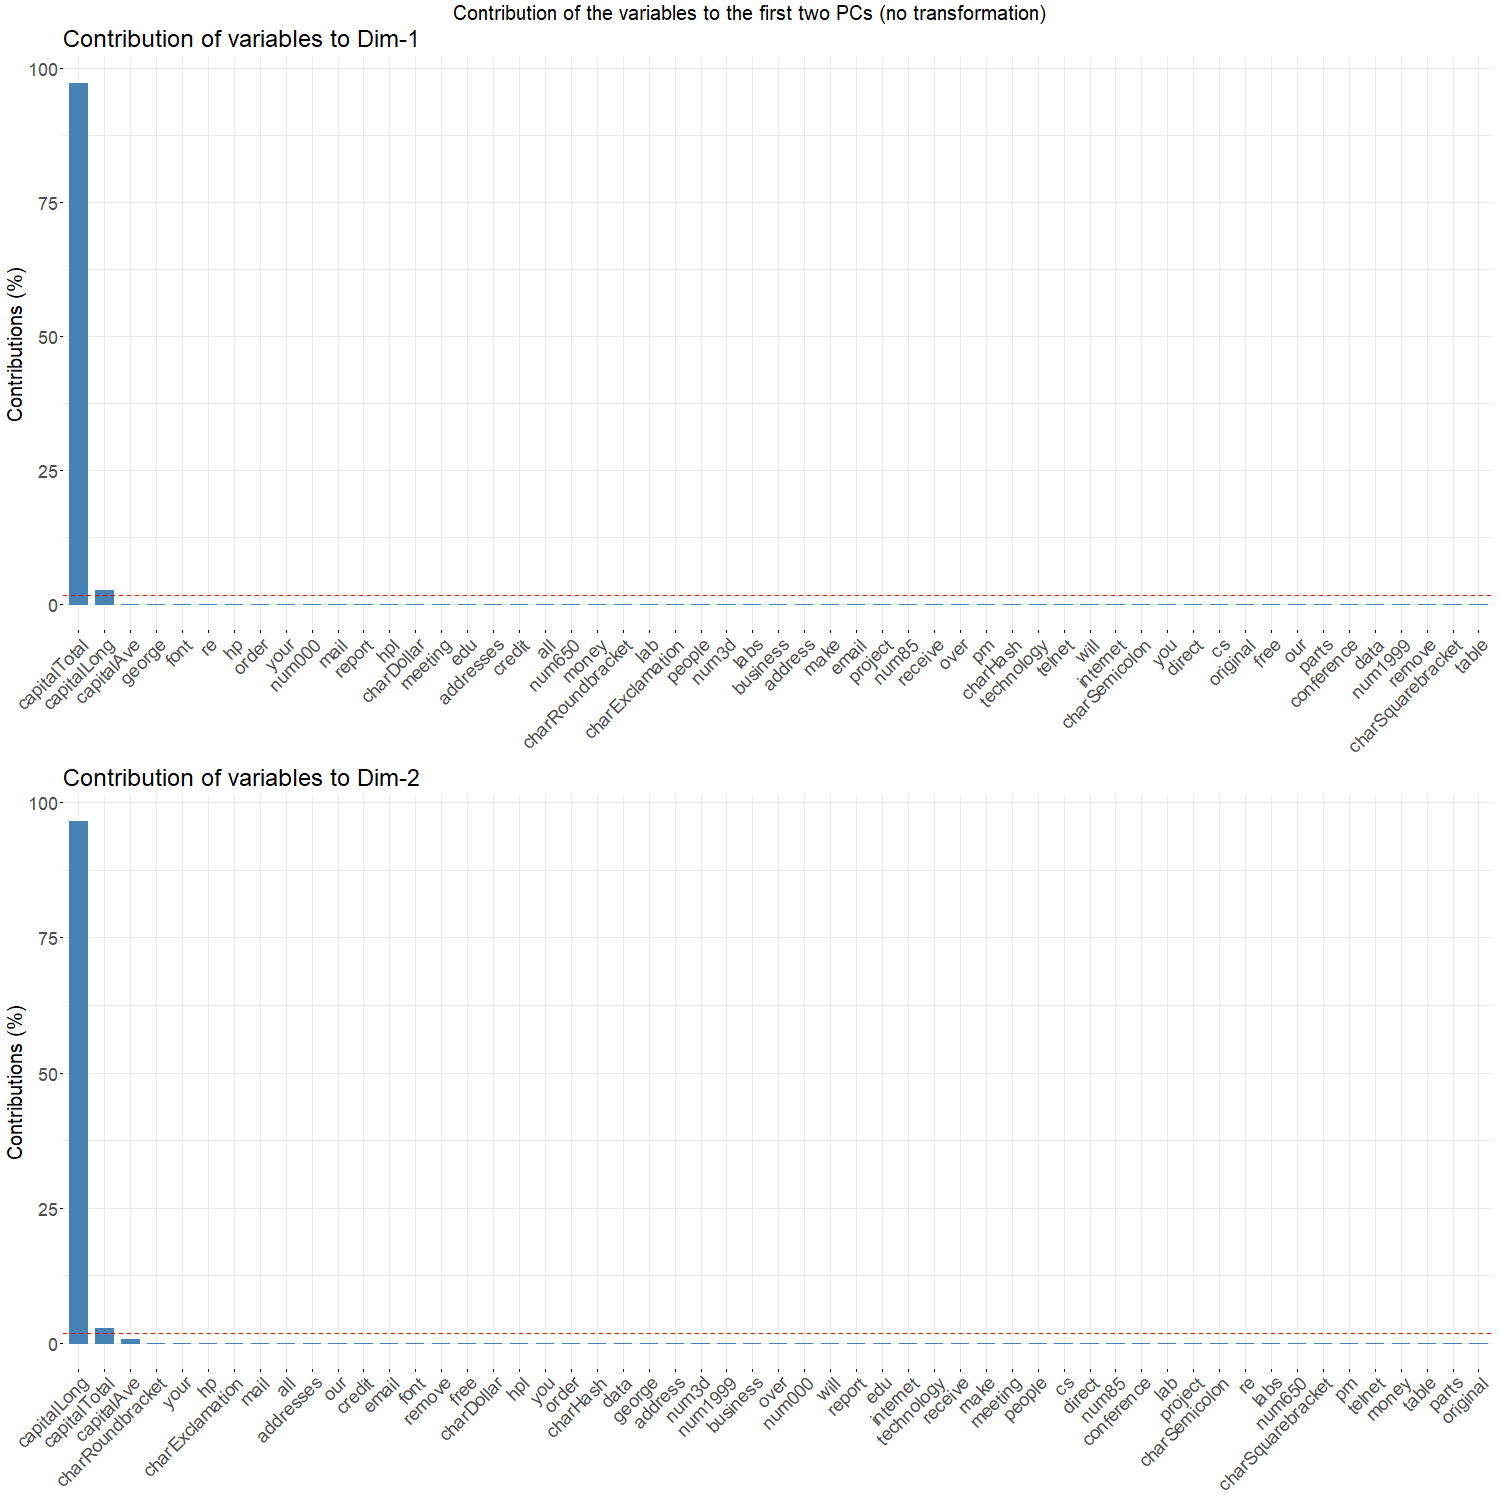
\includegraphics[width=0.7\textwidth]{"proj2_plots/varplot1.png"}
		\label{fig::varplot}
	\end{figure}
	
	As we expect the algorithm has poor quality as only variables with highest values are taken into consideration. In our data set most of the variables are frequencies with values in interval $[0, 100]$ and only capital letters characteristics have higher values. That causes the observed  behavior of PCA method, which results with only $2$ principal components, so in the following analyses we will use only transformed data.
	
	Let us now check the principal components for data after z-score standardization.
	
	\begin{figure}[h]
		\caption{PCA results for standardized data}
		\centering
		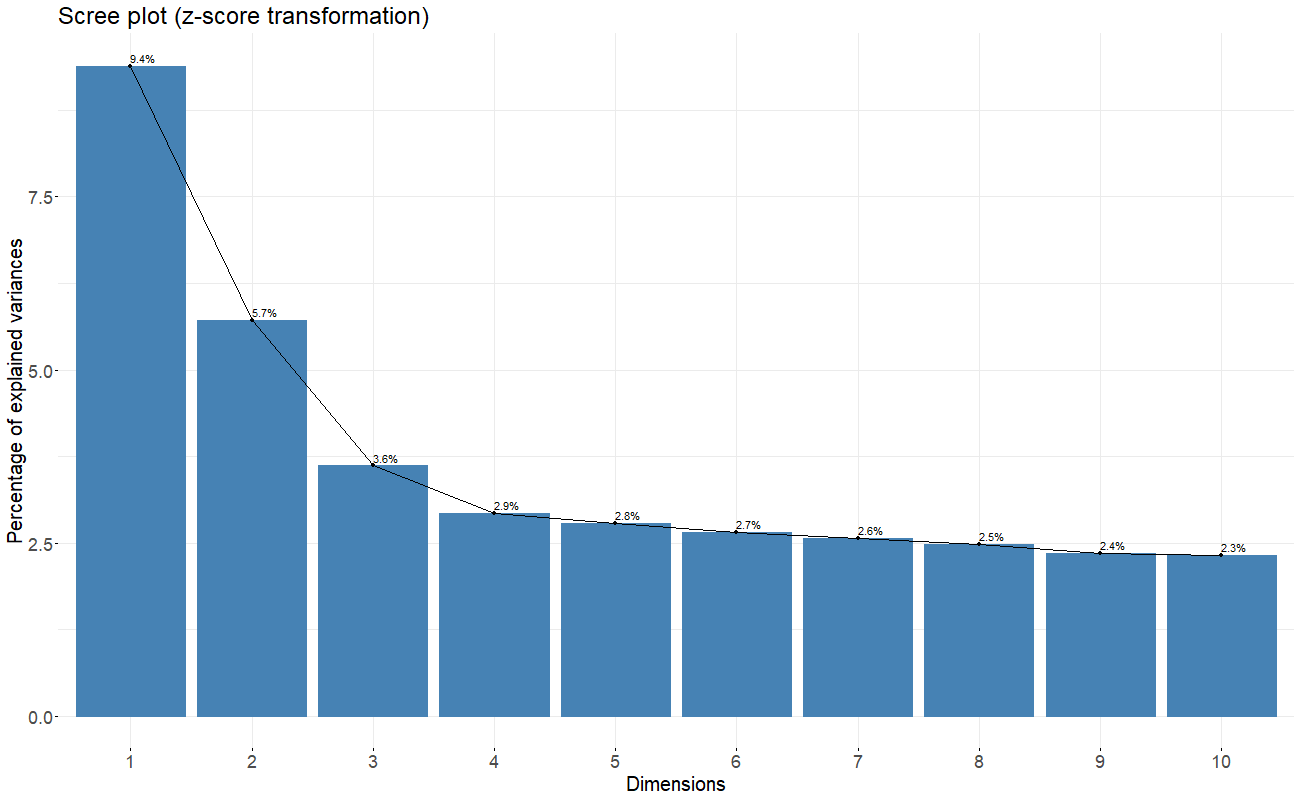
\includegraphics[width=0.7\textwidth]{"proj2_plots/screeplot2.png"}
		\label{fig::screeplot_zscore}
	\end{figure}
	
	\begin{figure}[h]
		\caption{PCA results for standardized data}
		\centering
		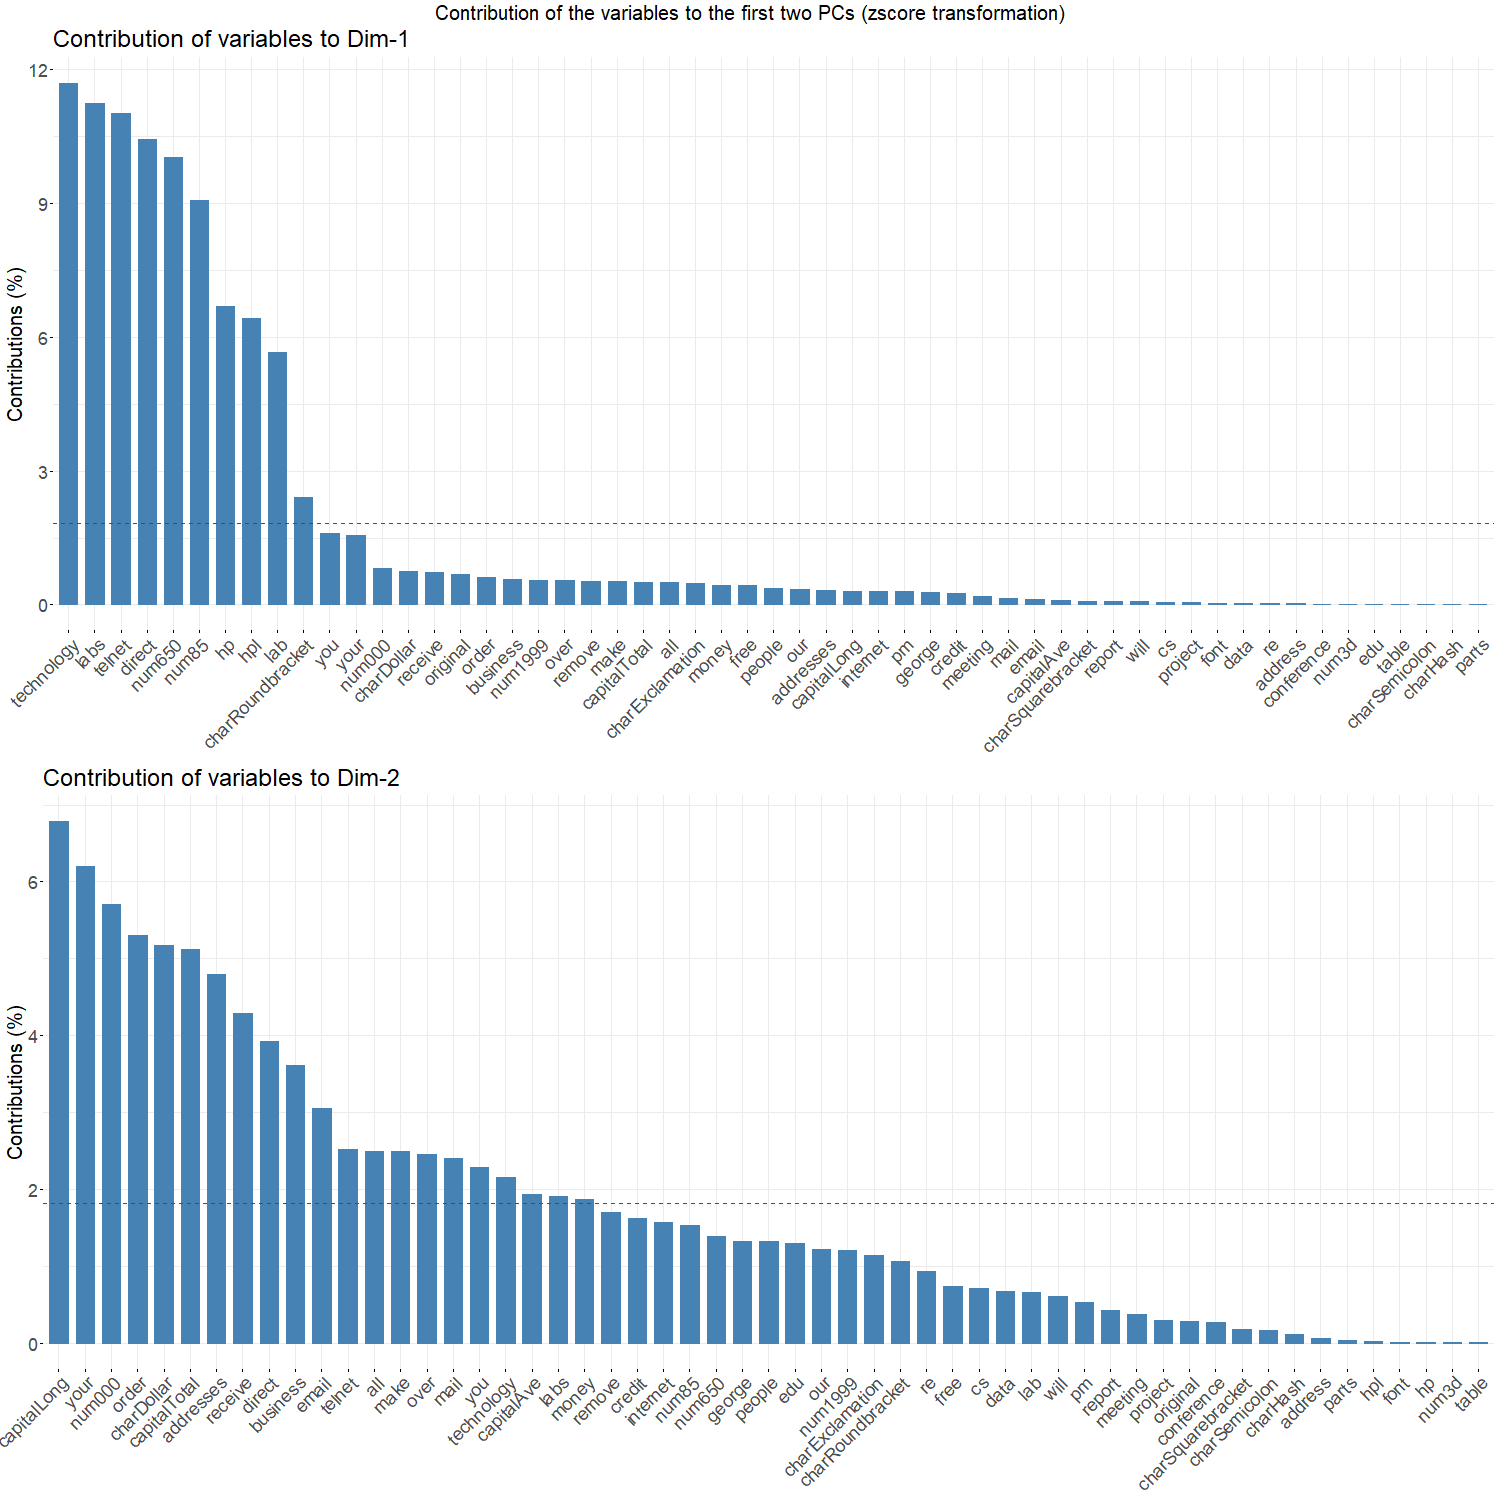
\includegraphics[width=0.7\textwidth]{"proj2_plots/varplot2.png"}
		\label{fig::varplot_zscore}
	\end{figure}
	
	As we anticipated in this case we get more principal components created and also increased number of features is taken into account.
	
	\begin{figure}[h]
		\caption{PCA results for log-transformed data}
		\centering
		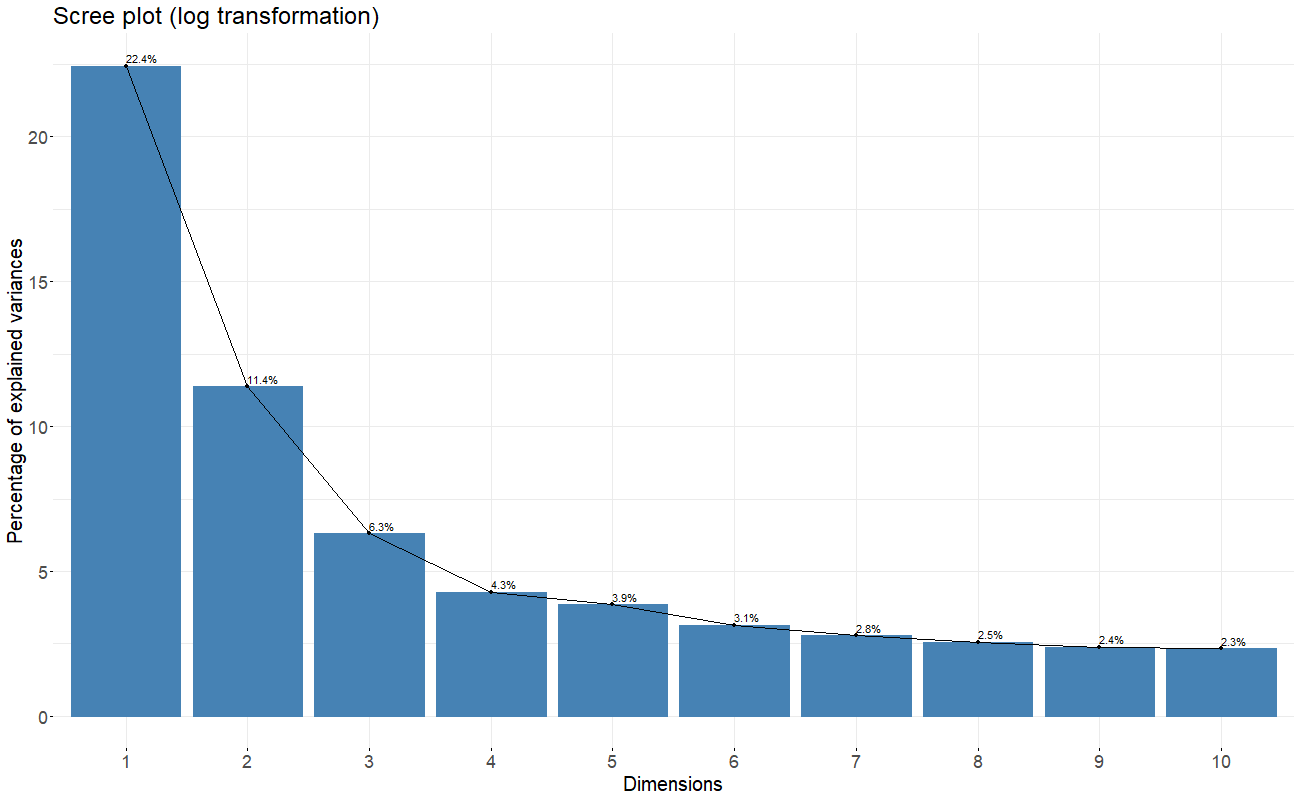
\includegraphics[width=0.7\textwidth]{"proj2_plots/screeplot3.png"}
		\label{fig::screeplot_log}
	\end{figure}
	
	\begin{figure}[h]
		\caption{PCA results for log-transformed data}
		\centering
		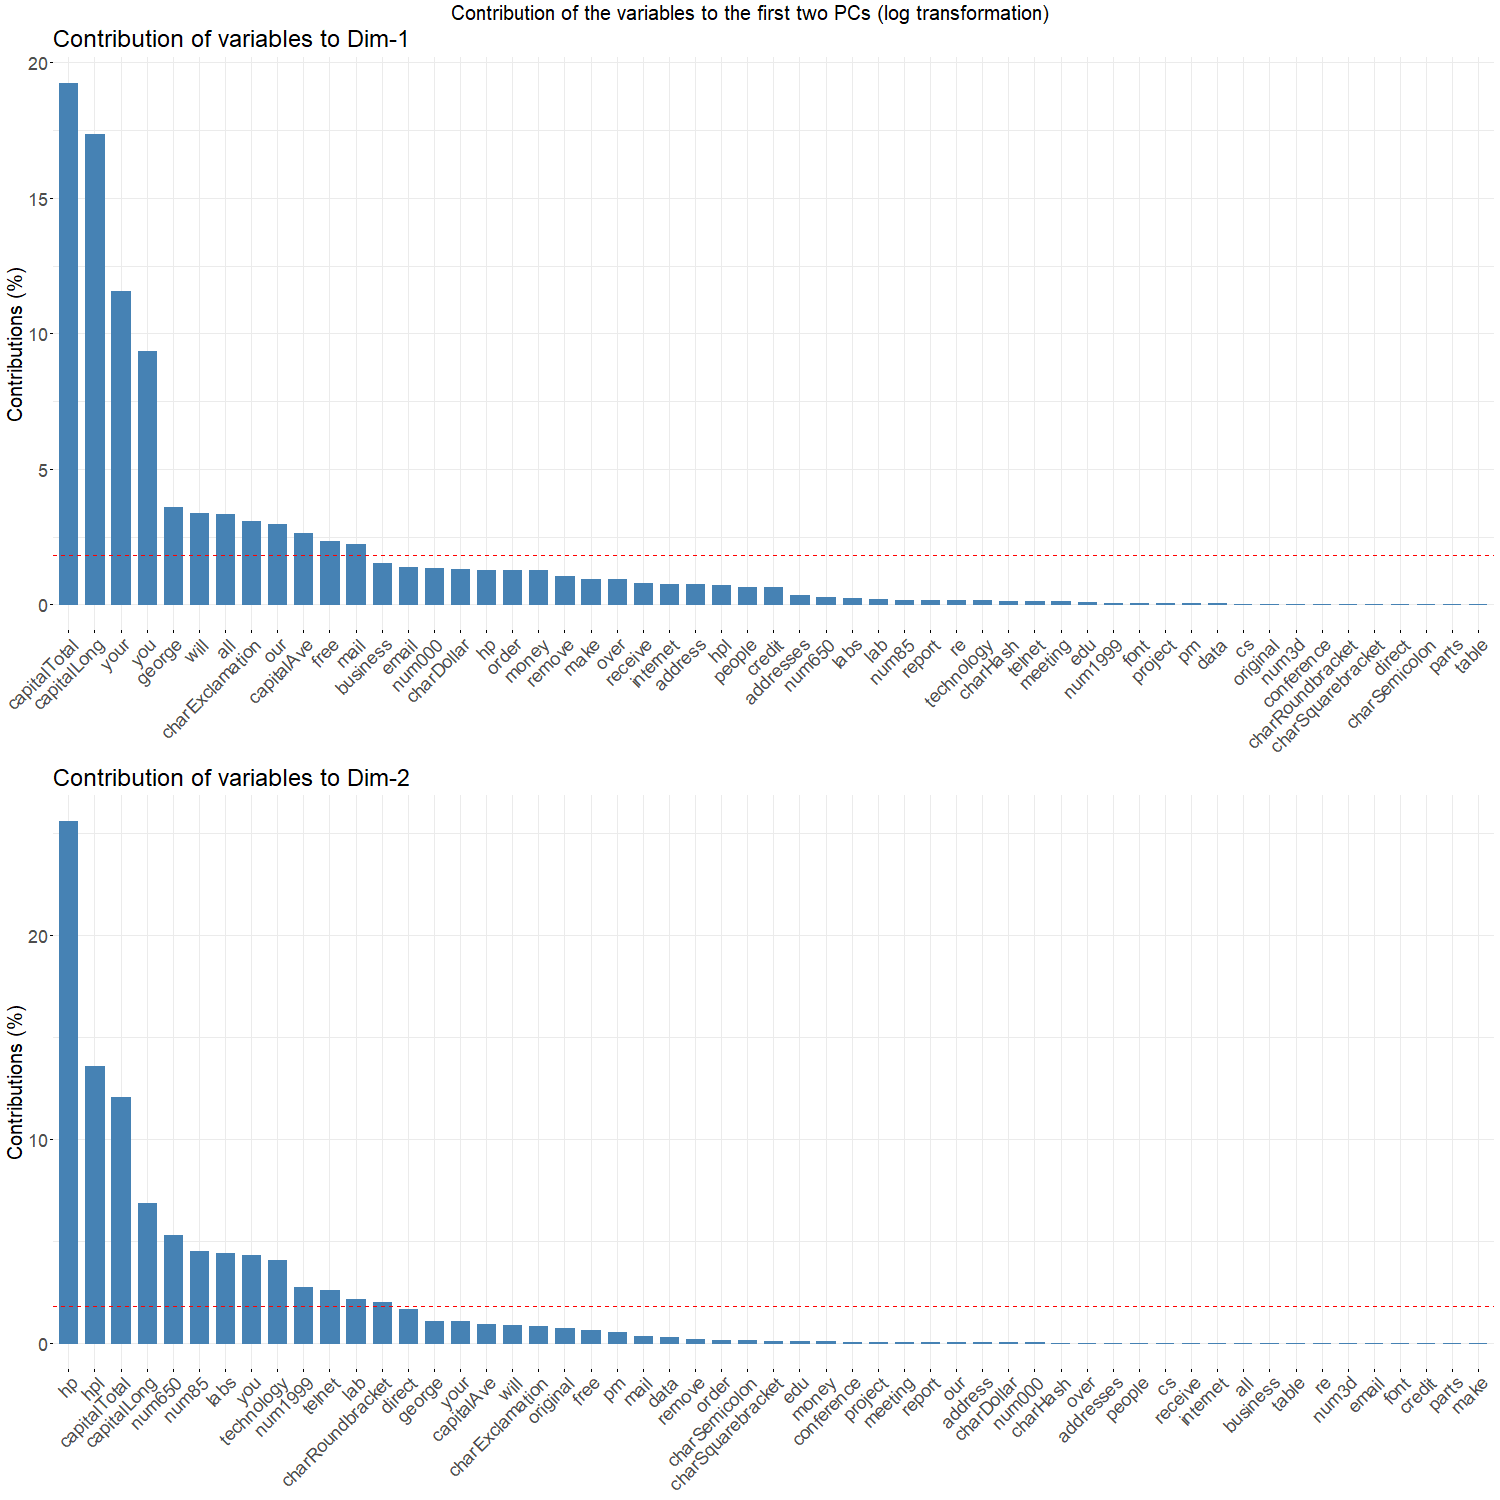
\includegraphics[width=0.7\textwidth]{"proj2_plots/varplot3.png"}
		\label{fig::varplot_log}
	\end{figure}
	
	Here again we observe that contribution of many variables is higher than for original data. Also we see that in comparison to z-score transformed data we will probably be able to eliminate more principal components for the latter analysis.
	
	\textbf{Add part about cutting PCs and method used, clean up plots}
	
	\section{Clustering}
	For clustering analysis we will use k-means, PAM and AGNES algorithms for transformed \textit{Spambase} data set and also for data set build using principal components extracted while performing PCA. 
	
	We are lucky to have the knowledge about number of classes in the examined data set (\textit{spam} and \textit{nonspam}), however let us check anyway if the number of clusters determined using \texttt{fviz\_nbclust} method is the same. On Figures \ref{fig::clust_num_kmeans},
	\ref{fig::clust_num_pam}, \ref{fig::clust_num_keans_pca} and \ref{fig::clust_num_pam_pca} we present the results for k-means and PAM algorithms.
	
	\begin{figure}[h]
		\caption{Number of clusters for k-means (no PCA)}
		\centering
		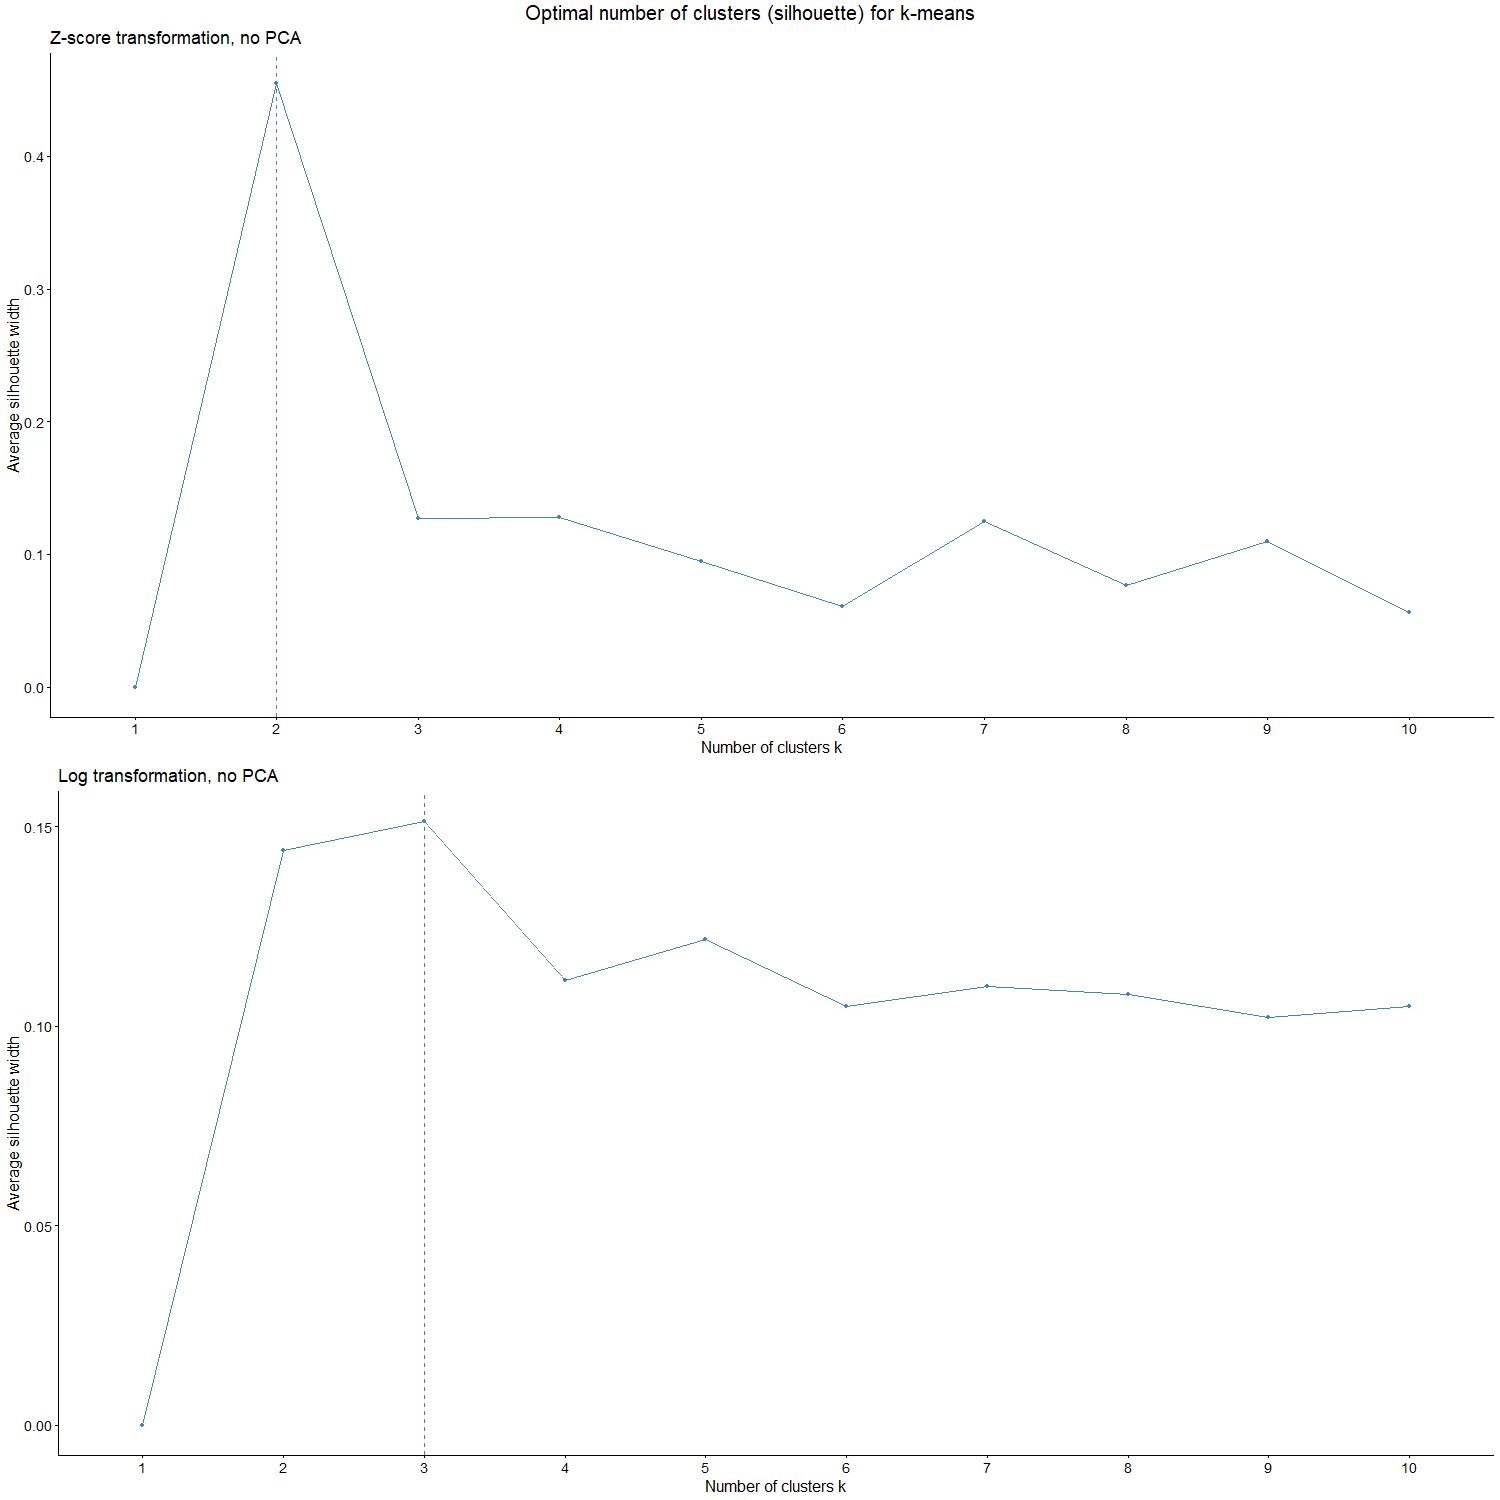
\includegraphics[width=0.5\textwidth]{"proj2_plots/kmeans_clust_num.png"}
		\label{fig::clust_num_kmeans}
	\end{figure}
	
	\begin{figure}[h]
		\caption{Number of clusters for pam (no PCA)}
		\centering
		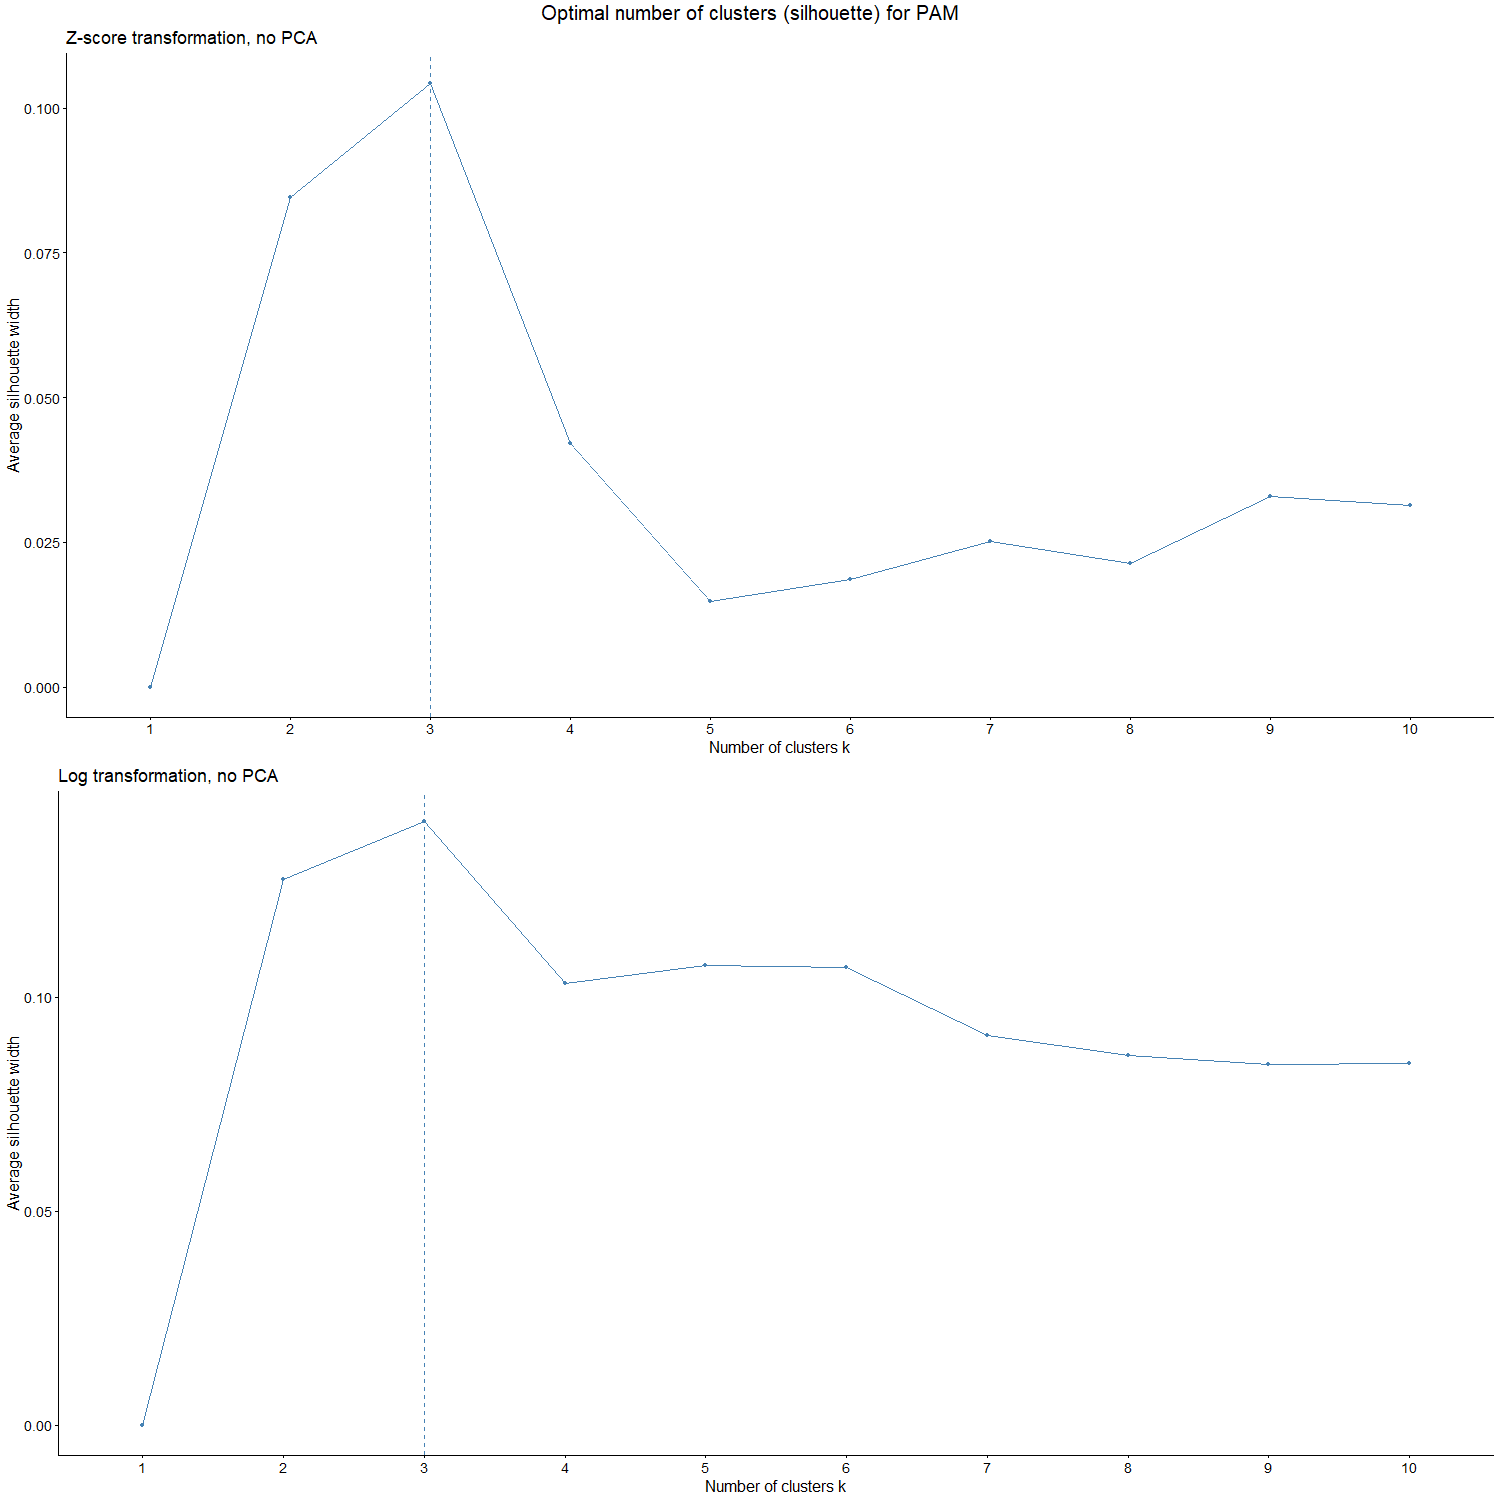
\includegraphics[width=0.5\textwidth]{"proj2_plots/pam_clust_num.png"}
		\label{fig::clust_num_pam}
	\end{figure}
	
	\begin{figure}[h]
		\caption{Number of clusters for k-means (with PCA)}
		\centering
		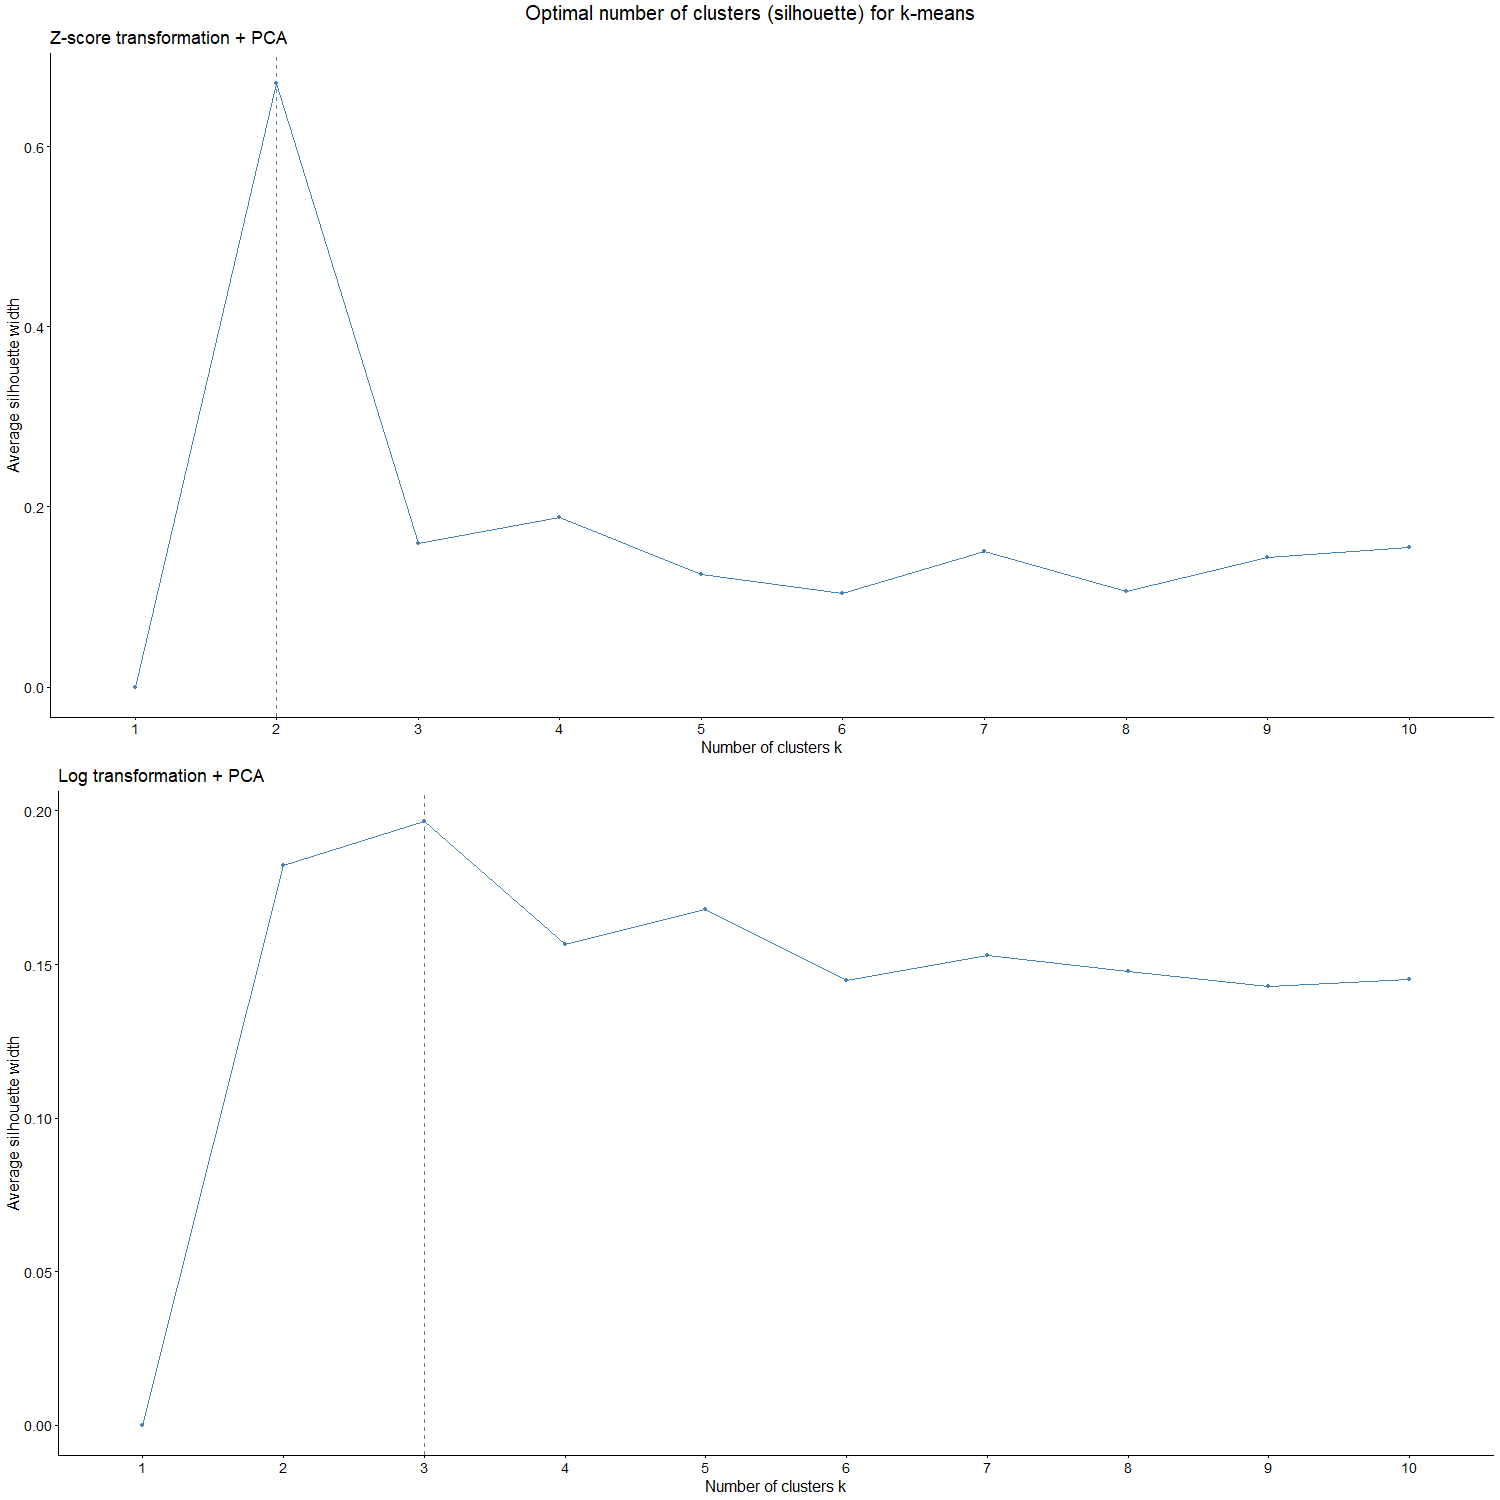
\includegraphics[width=0.5\textwidth]{"proj2_plots/kmeans_clust_num_pca.png"}
		\label{fig::clust_num_keans_pca}
	\end{figure}
	
	\begin{figure}[h]
		\caption{Number of clusters for pam (with PCA)}
		\centering
		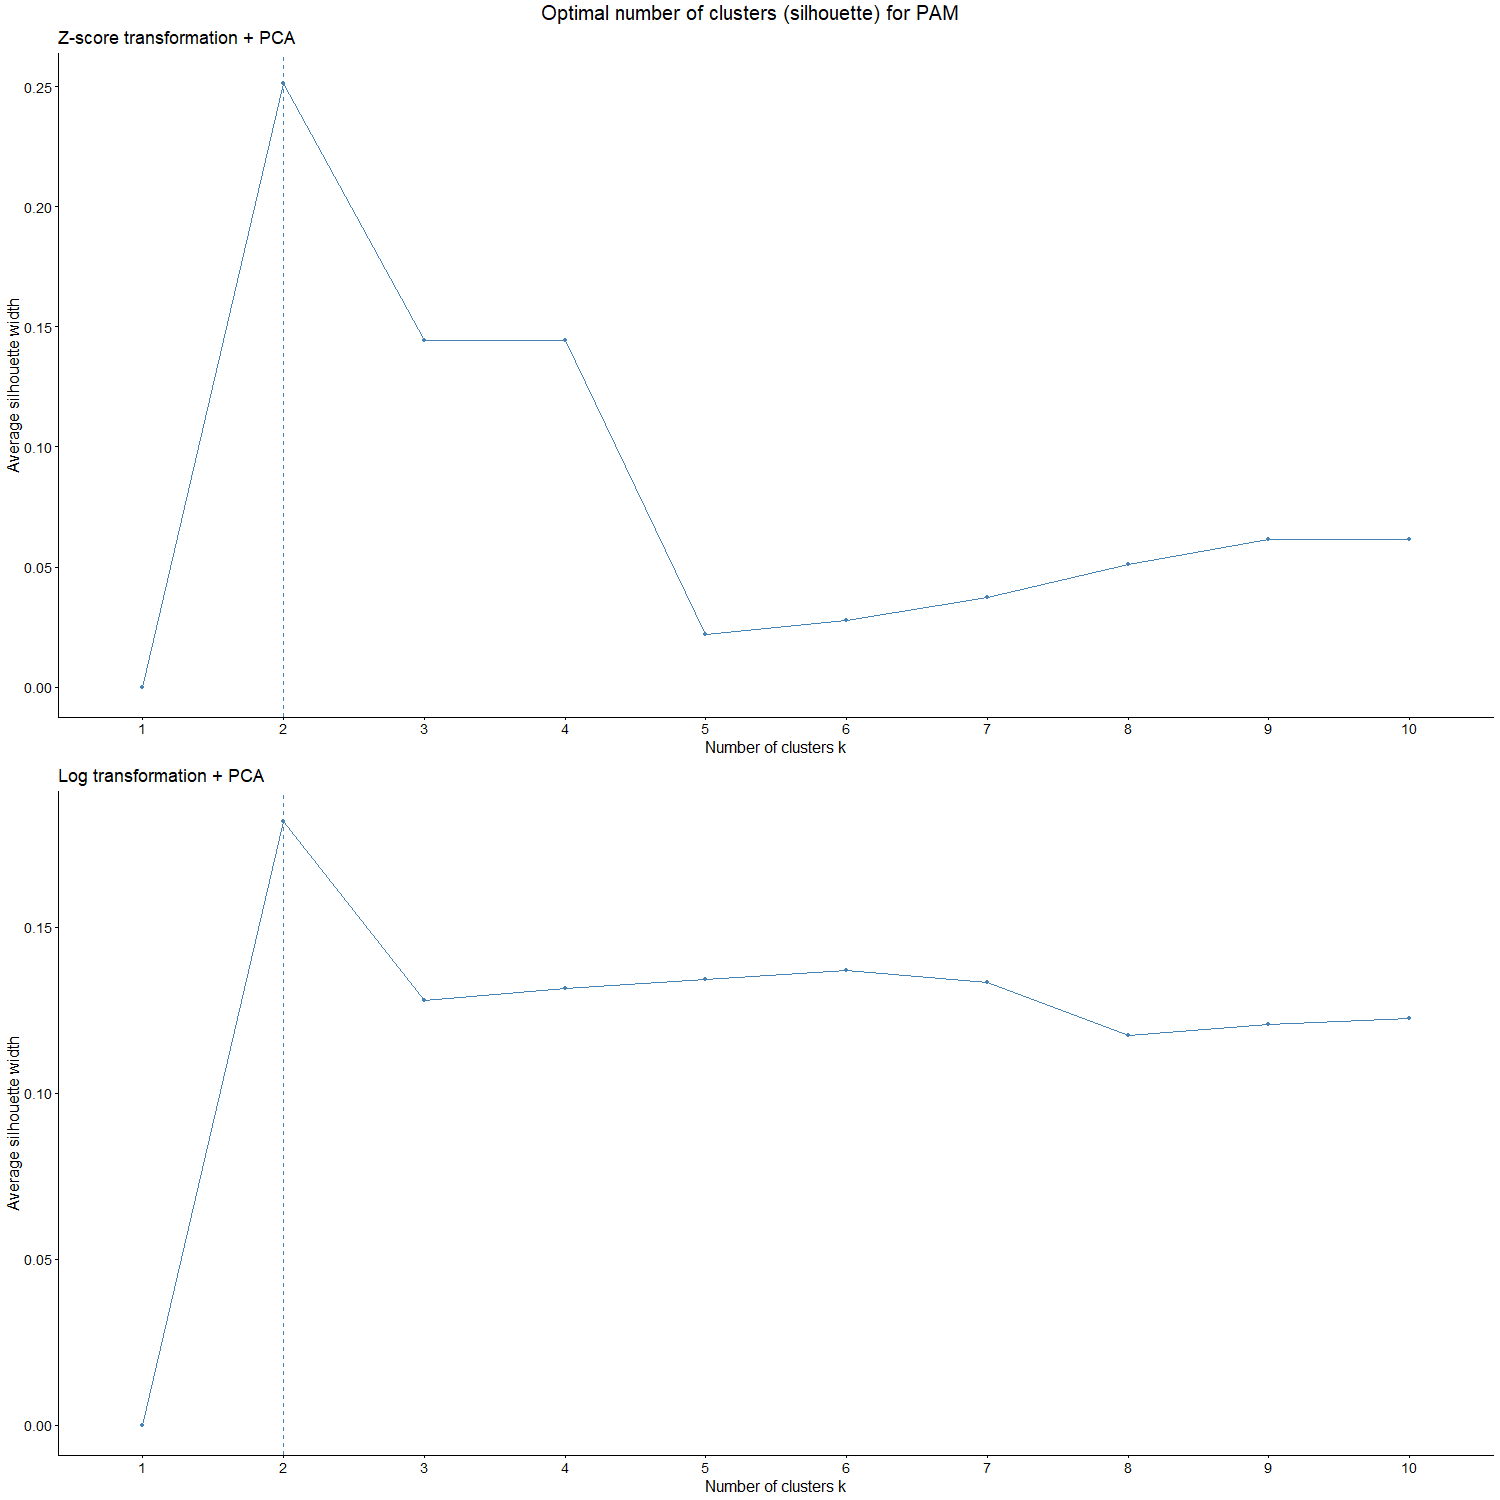
\includegraphics[width=0.5\textwidth]{"proj2_plots/pam_clust_num_pca.png"}
		\label{fig::clust_num_pam_pca}
	\end{figure}
	
	In all cases the estimated number of clusters is equal to or one more that the actual number of clusters. It means that we should assume that number of clusters is $2$ or $3$, but considering the knowledge about used data set, we will assume two clusters in each algorithm to be able to compare the data partition with classification results.
	
	For AGNES the method to establish the number of clusters is not that straightforward. Here we need to use dendrograms, that will enable us to determine number of clusters. This algorithm also allows us to find outliers in the data set, that are not associated with any cluster.
	
	
	\subsection{k-means}
	
	\subsection{PAM}
	
	\subsection{AGNES}
	 
\end{document}